\section{Nuclear Recoil Equivalent Energy Scale}
\label{secLeff}


In liquid xenon based experiments, the nuclear recoil equivalent energy scale is determined based on the scintillation signal S1~\cite{xe10-independent, NR_Zeplin}, however, it has been suggested to use the combined energy for this purpose~\cite{CESshutt}. Electronic and nuclear recoils produce different amounts of the scintillation light and ionization electrons because of their different $dE/dx$ behavior (see Section~\ref{secDetectionPrinciple}). Since the measurement of the absolute scintillation efficiency for nuclear recoils is very difficult, the scintillation yield of the liquid xenon detectors is commonly calibrated relative to the one of electronic recoils of 122~keV $\gamma$-rays from a $^{57}$Co source. The scintillation yield of nuclear recoils relative to that of 122~keV $\gamma$-rays is called the relative scintillation efficiency ($L_{eff}$) and is used to define the nuclear recoil equivalent energy scale, based on the know light yield at 122~keV.

\begin{figure}[!b]
\centering
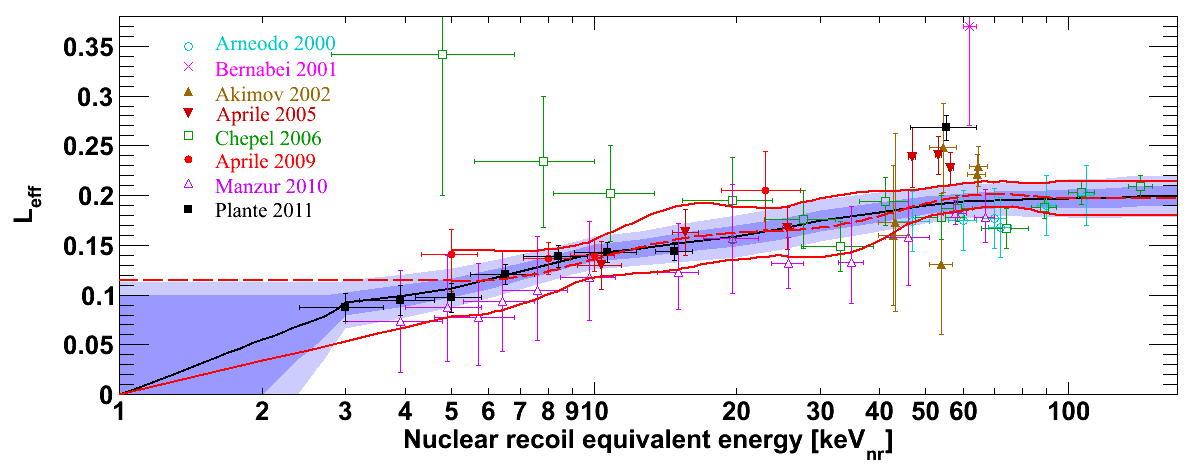
\includegraphics[width=1.0\linewidth]{plots/run08/run08_Leff_mod1.png}
\caption[All direct measurements of $L_{eff}$ and the parametrization used for analysis of the XENON100 data]{All direct measurements of $L_{eff}$ and the parametrization used for analysis of the XENON100 data. 
The red dashed and solid lines show the global fit to the measurements between 5~keV$_{\mathrm{nr}}$ and 100~keV$_{\mathrm{nr}}$, and 90\% confidence contour, respectively. The lower 90\% contour has been extrapolated to zero scintillation at 1~keV$_{\mathrm{nr}}$. 
The black solid black line shows the mean of the distribution described by a Gaussian function, including the latest $L_{eff}$ measurements~\cite{LeffPlante} shown by black squares. The shaded blue regions show 1$\sigma$ and 2$\sigma$ of the uncertainty band. Below 3~keV$_{\mathrm{nr}}$ the trend is logarithmically extrapolated to L$_{eff}$~=~0 at 1~keV$_{\mathrm{nr}}$. }
\label{figLeffRun08}
\end{figure}

$L_{eff}$ can be inferred indirectly from a comparison of neutron calibration spectra with Monte Carlo simulations~\cite{LeffSorensen, LeffZeplin, LeffZeplinHorn}, or directly measured at fixed neutron energies~\cite{LeffArneodo, LeffBernabei,  LeffAprile2005, LeffChepel, LeffAprile2009, LeffManzur, LeffPlante}. The latter, shown in Fig.~\ref{figLeffRun08}, have less systematic uncertainties and have been used to define the nuclear recoil equivalent energy for the analysis of the XENON100 data.

The energy dependence of $L_{eff}$ and its uncertainly have been determined from the measured data points shown in Fig.~\ref{figLeffRun08} through a global cubic-spline fit in the energy range from the lowest energy data point to 100~keV$_{\mathrm{nr}}$. The measurements from Ref.~\cite{LeffPlante} with the lowest uncertainty have not been available for the analysis of the data acquired in the commissioning run in Fall 2009 (run07 \cite{xe100-run07}). The spline knots have been fixed at 5, 10, 25, 50, and 100~keV$_{\mathrm{nr}}$. A constant extrapolation of $L_{eff}$ below 5~keV$_{\mathrm{nr}}$ has been used, with the 90\% confidence level contour logarithmically extrapolated to zero scintillation yield at 1~keV$_{\mathrm{nr}}$.

For the analysis of the first science run data (run08 \cite{xe100-run08}), the data point at 3~keV$_{\mathrm{nr}}$ has been included in the global fit for analysis, and the lowest spline knot has been fixed at 3~keV$_{\mathrm{nr}}$. 
Below the lowest measured energy of 3~keV$_{\mathrm{nr}}$, $L_{eff}$ has been logarithmically extrapolated to zero.

The nuclear recoil energy in [keV$_{\mathrm{nr}}$] is inferred from the S1 signal via:
\begin{equation}
E_{\mathrm{nr}} = \frac{ \mathrm{S}1 \cdot S_{\mathrm{ee}} }{ L_{y} \cdot L_{eff} \cdot S_{\mathrm{nr}} },
\end{equation}
where $L_{y}$ = (2.20$\pm$0.09)~PE/keV$_{\mathrm{ee}}$ - light yield for 122~keV$_{\mathrm{ee}}$ electronic recoils, $L_{eff}$ - scintillation efficiency for nuclear recoils relative to that for 122~keV $\gamma$-rays, $S_{\mathrm{ee}}$ = 0.58~\cite{FieldQuenchingFactorsAprile} - scintillation quenching factor due to electric field for electronic recoils, $S_{\mathrm{nr}}$~=~0.95~\cite{FieldQuenchingFactorsAprile} - electric field quenching factor for nuclear recoils. 
Due to the short mean free path of 122~keV $\gamma$-rays in liquid xenon ($\sim$2~mm), they cannot penetrate far into the target volume. Therefore, their light yield $L_{y}$ at the drift field of 530~V/cm has been extrapolated from a fit to $\gamma$-lines with higher energies. 




%The energy calibration for nuclear recoils 


%\begin{figure}[!h]
%\centering
%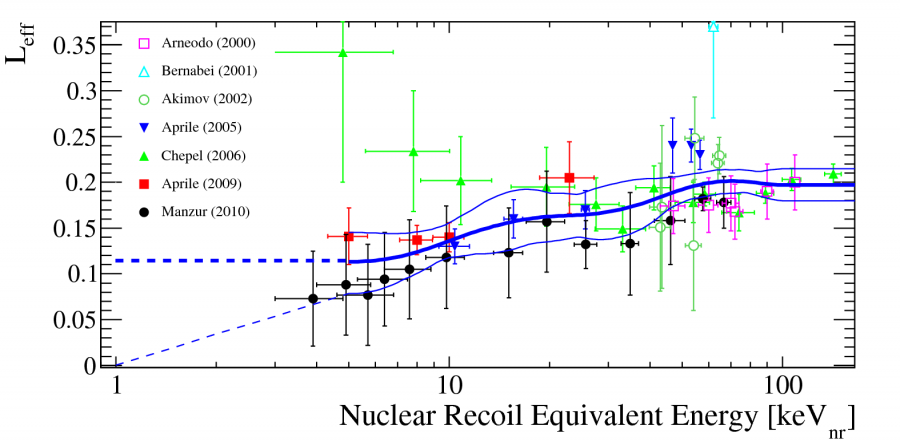
\includegraphics[width=1.0\linewidth]{plots/run07/run07_Leff.png}
%\caption{}
%\label{figLeffRun07}
%\end{figure}


